\documentclass{article} % For LaTeX2e
\usepackage{nips13submit_09,times}
\usepackage{hyperref}
\usepackage{url}
\usepackage{graphicx}

% \setlength{\headwidth}{6.40in}
% \addtolength{\textwidth}{1in}
% \addtolength{\textheight}{1in}
% \addtolength{\evensidemargin}{0.5in}
% \addtolength{\oddsidemargin}{-0.5in}
% \addtolength{\topmargin}{-0.5in}

\newcommand{\argmax}{\arg\!\max}
\newcommand{\argmin}{\arg\!\min}
% \newcommand{\argmax}{\operatornamewithlimits{argmax}} % need \usepackage{amsmath}
% \DeclareMathOperator*{\argmax}{arg\,max}

\setlength\parindent{0pt}

\title{\bf Logistic Regression with L$_2$ Regularization}
\author{\textbf{Sandy Wiraatmadja}\\
swiraatm@eng.ucsd.edu
\And
\textbf{Qiheng Wang}\\
qiw018@cs.ucsd.edu}

\newcommand{\fix}{\marginpar{FIX}}
\newcommand{\new}{\marginpar{NEW}}

\nipsfinalcopy % Uncomment for camera-ready version

\begin{document}

\maketitle


\begin{abstract}
In this paper, we explore logistic regression with $L_2$ regularization as a binary classification learning model. Given a set of data with different feature values, we want to be able to closely predict what the binary label is for each example. This can be done by training the model on a training set to find the parameters that maximize its log conditional likelihood (LCL). Two optimization methods are analyzed in this paper: Stochastic Gradient Descent (SGD) and Limited-memory BFGS (L-BFGS). The two methods are applied to the Gender Recognition [DCT] dataset from MLcomp \cite{DCTdata}. Logistic regression with SGD produces test accuracy averaging at 0.9164, which is just a little higher than L-BFGS test accuracy with an average of 0.9123.


\end{abstract}


%-----------------------------------------------------------------------------
% INTRODUCTION
%-----------------------------------------------------------------------------
\section{Introduction}
\label{sec:intro}

Machine learning, which is a branch of artificial intelligence, has been growing significantly due to the availability of massive data that can be used in developing and training models. One common problem in machine learning is to train a model that can be used for binary statistical classification. For example, given a data of email messages, some classified as spam and some as non-spam, a model can be trained to learn some distinguishing features between spam and non-spam emails. After the learning process is done and the parameters are chosen, the model can be used on a new data of email messages to label each email as either spam or non-spam. Several classifier learning algorithms have been developed throughout the years, such as k-nearest neighbors, linear regression, or support vector machines \cite{wiki_classifier}. One particular algorithm that we focus on in this paper is logistic regression.

%% TODO: Add more about logistic regression. How it works (no algorithm here). Just talking about how
%% it tries to fit the training data to find the parameters tha maximizes the log joint conditional likelihood. In order to find
%% the maximum  likelihood, we compare 2 optimization algorithm: our implementation of sgd and Mark Schmidt's
%% implementation of l-bfgs.

Logistic regression model is widely used in probabilistic classification by fitting the training data to the model and find the parameters that maximizes the log joint conditional likelihood (LCL) of the training set.
In this paper, we analyze how to train a logistic regression model for our binary (Bernoulli) label classification problem with two different gradient-based optimization methods for maximizing the LCL\@.
These two algorithms are Stochastic Gradient Descent (SGD) which uses a modified version of a gradient descent method, and Limited-memory Broyden-Fletcher-Goldfarb-Shanno (L-BFGS) which uses the quasi-Newton methods \cite{wiki_lbfgs}.
We use our own implementation of the SGD algorithm in Matlab, while on the other hand, we used Mark Schmidt's Matlab {\tt minFunc} function which implemented L-BFGS \cite{minFunc}.
We compare the two models to see how well they perform on the Gender Recognition [DCT] test set from MLcomp.

%-----------------------------------------------------------------------------
% DESIGN AND ANALYSIS OF ALGORITHMS
%-----------------------------------------------------------------------------
\section{Design and Analysis of Algorithms}
\label{sec:algorithms}


%% TODO: Here I want to talk about the objective  function: maximize LCL.Explain about why we want to use
%% regularization to minimize overfitting -- show the RLCL function and Beta. And then we create 2 sections: SGD and L-BFGS.

Logistic regression uses the principle of maximum log conditional likelihood, where we choose a parameter estimate $\hat{\theta}$ that maximizes the log joint conditional likelihood \cite{elkan}. This is the sum of the log conditional likelihood for each training example:
\begin{eqnarray}
\label{LCL}
LCL &=& \sum_{i=1}^{n} \log L(\theta;y_i|x_i) = \sum_{i=1}^{n} \log f(y_i|x_i;\theta) \nonumber \\
    &=& \sum_{i:y_i=1} \log p_i + \sum_{i:y_i=0} \log (1-p_i) \nonumber \\
    &=& \sum_{i=1}^{n} \log (p_iy_i +(1-p_i)y_i).
\end{eqnarray}
Here we assume the conditional model
\begin{equation} \label{eq:p_i_alpha_beta}
p_i = p(Y=1|x;\alpha,\beta) = \sigma(\alpha + \sum_{j=1}^{d}\beta_{j}x_j) = \frac{1}{1+\exp-[\alpha+\sum_{j=1}^{d}\beta_{j}x_j]}
\end{equation}
where $\alpha$ is the intercept. For simplification, we assume that $\alpha = \beta_0$ and we add $x_0 = 1$ for all examples, such that (\ref{eq:p_i_alpha_beta}) becomes
\begin{equation} \label{eq:p_i}
p_i = \frac{1}{1+\exp-[\sum_{j=0}^{d}\beta_{j}x_j]}.
\end{equation}
The objective function of the logistic regression model is to find the parameter vector $\hat{\beta}$ such that
\begin{equation} \label{eq:objfun}
\hat{\beta} = \argmax_{\beta} LCL.
\end{equation}

Since logistic regression tries to fit the training data into the model to maximize LCL, the problem of overfitting tend to arise.
In one extreme example, parameters could be sent to $\pm \infty$ with either a monotonically positive or negative gradient of LCL\@.
The standard method to solve this problem is by introducing regularization to the model, which imposes a penalty on the magnitude of the parameter values.
However, there is a tradeoff between minimizing the regularization penalty and maximizing the regularized log joint conditional likelihood (RLCL).
With the added regularization penalty, the objective function for the optimization problem becomes
\begin{equation} \label{eq:objfun_reg}
\hat{\beta} = \argmax_{\beta} RLCL = \argmax_{\beta} (LCL - \mu ||\beta||_2^2)
\end{equation}
where $||\beta||_2^2 = \sum_{j=1}^{d} \beta_j^2$ is the squared $L_2$ norm of the parameter vector $\beta$ of length $d$. The constant $\mu$ is the strength of the regularization which quantifies the trade-off between maximizing likelihood and minimizing parameter values, preventing those parameters from going to infinity. This is called the quadratic or Tikhonov regularization. Note that since each training data provides information about the intercept of the model $\beta_0$, there is enough information to avoid overfitting of this parameter. Therefore, $\beta_0$ does not need to be regularized \cite{elkan}.

The partial derivative of LCL with respect to parameter $\beta_j$ is
\begin{equation} \label{eq:d_LCL}
\frac{\partial}{\partial \beta_j} LCL = \sum_i(y_i-p_i)x_{ij}
\end{equation}
whereas the partial derivative of RLCL with respect to parameter $\beta_j$ is
\begin{equation} \label{eq:d_RLCL}
\frac{\partial}{\partial \beta_j} RLCL = \sum_i(y_i-p_i)x_{ij} - 2 \mu \beta_j.
\end{equation}
The following subsections discuss the different algorithm of the two optimization methods.


\subsection{Stochastic Gradient Descent}
% TODO:   We are actually doing stochastic gradient ascent here since we want to maximize
% the objective function -- so Beta := Beta + ...
% Talk a little bit about the iteration (give the update formula). Convergence checking done only after each epoch,
% done by checking the difference between the RLCL values between one epoch to the next. The learning rate lambda
% is made smaller after every epoch by 10%, to have better convergent point and to converge faster.

Since our objective function is a maximization problem, this method should be more appropriately called the stochastic gradient ascent. The parameter values $\beta$ is changed one step at a time following the gradient until it finally converges to the local maxima point.

The regular gradient descent update rule of the parameter $\beta_j$ is
\begin{equation} \label{eq:update_rule_regular}
\beta_j := \beta_j + \lambda \frac{\partial}{\partial \beta_j} RLCL
\end{equation}
where $\lambda$ is the learning rate, denoting how big of a step each update should take. However, calculating the partial derivatives per iteration can be time consuming as each requires $O(nd)$ time where $n$ is the training example size and $d$ is the number of features.

To minimize computation, we use stochastic gradient descent method, where we get a random approximation to the partial derivatives by just looking at one randomly chosen example at a time to update $\beta$. Thus, we can calculate it in much less time, around $O(d)$ time, independent of the size of the training data. This is extremely useful for very large training set.

By using SGD, the parameter update rule then becomes
\begin{equation} \label{eq:update_rule_stochastic_i}
\beta_j := \beta_j + \lambda [(y_i - p_i)x_j - 2 \mu \beta_j]
\end{equation}
for any randomly chosen $i^{th}$ example. And the update rule for the whole parameter vector $\bar{\beta}$ is
\begin{equation} \label{eq:update_rule_stochastic}
\bar{\beta} := \bar{\beta} + \lambda (\bar{y} - \bar{p})^{T}X
\end{equation}
This vector update should be done at least once after each epoch of stochastic gradient ascent iteration. An epoch is a complete update for every example in the dataset.

Convergence is reached when the change in the objective value, RLCL, is within a certain threshold which we hold constant at $10^{-3}$. Typically, this check is done in the middle of an epoch, which means that the iteration can stop if it reaches convergence before even going through the entire examples. This can save a lot of time when dealing with massive data. However, we decided to do the convergence check after every epoch. The learning rate $\lambda$ is made smaller by 10\% after every epoch. This is done so that convergence is reached faster. Additionally, bigger $\lambda$ means bigger step and this might cause instability where the objective function cannot reach its true local maxima.


\subsection{L-BFGS}
%% L-BFGS: the minFunc function is minimizing so we do Beta := Beta - ... and the objective function becomes
%% Beta = argmin -LCL + ...
%% include some wiki information on this

L-BFGS is an optimization algorithm of the quasi-Newton method using a limited amount of computer memory\cite{wiki_lbfgs}. This method is often used for parameter estimation. As mentioned above, for the purpose of this paper, we use Mark Schmidt's {\tt minFunc} function, written in Matlab, that implements the L-BFGS algorithm. This function is a minimizing function. Therefore, for consistency, we modify the objective function (\ref{eq:objfun_reg}) from maximizing the regularized LCL to minimizing its negative value.
\begin{eqnarray} \label{eq:objfun_reg_minimize}
\hat{\beta}&=&\argmin_{\beta} (- RLCL) \nonumber \\
           &=&\argmin_{\beta} (- LCL + \mu ||\beta||_2^2)
\end{eqnarray}


%-----------------------------------------------------------------------------
% DESIGN OF EXPERIMENTS
%-----------------------------------------------------------------------------
\section{Design of Experiments}
\label{sec:experiments}


%% TODO: talk about the implementation:
% in matlab, using the dataset from gender recognition (559 training, 239 test, 800 features).
% 1. Preprocess data -- normalize to mean zero and unit variance. make sure to use the same normalization factor on test data
% 2. Randomize order of training set
% 3. split training data: 80% training (447 samples, train param Beta), 20% validation (112 samples, train hyperparameters)
% the hyperparameters are chosen using grid search. For SGD there are 2: mu and lambda (10^-10, 10^-9, ..., 10^10)
% For L-BFGS, there is only one hyperparam: mu (10^-10, 10^-9,..., 10^10).
% 4. Use intialization Beta = 0
% 5. Max epoch = 100
% 6. Use checkgrad to verify that our derivatives are correct

The stochastic gradient descent and L-BGS methods, both implemented in Matlab, are tested on the Gender Recognition [DCT] dataset from MLcomp, which contains 559 training examples and 239 test examples, with 800 features and a binary label. However, we need to have a separate set for validation, to choose the hyperparameter values that best fits our model on the training set. Therefore, we split the training set such that 80\% of it becomes the training set, consisting of 447 samples, and the other 112 samples will be the validation set.

First, we preprocess the dataset by normalizing the feature values using z-scoring method such that each feature has zero mean and unit variance. The same normalization factors, calculated from the training data, are used in the testing set as well. For simplicity, we also change the label values from -1 to 0, so that the binary label value becomes 0 or 1, instead of -1 or 1. We then add a column of ones in front of both the training and testing dataset, to correspond to the intercept term that is added to the parameter $\beta$ as seen in (\ref{eq:p_i}).

Secondly, we randomize the order of the training set. This is not required for the L-BFGS implementation since it reads the entire training set at every iteration. However, with stochastic gradient descent, the order of the training data becomes more significant. Later data in the epoch tend to have more impact on the model. This randomization of training set is done to guarantee that the data is not originally sorted in any way that might affect the learning process.

The hyperparameters for both models are chosen using the grid search method. For stochastic gradient descent, there are two hyperparameters to be trained, which are the regularization strength $\mu$ and the learning rate $\lambda$. The grid search for both parameters is done over the range of \{$10^{-5},$ $10^{-4}$, \ldots, $10^5$\}. Different combinations of $\lambda$ and $\mu$ are tried on the training set to train the model and the combination that gives highest accuracy in the validation set is picked. The same grid search is done for the L-BFGS model, however there is only one hyperparameter to be trained here, namely the regularization strength $\mu$. This is done over the same range of \{$10^{-5}$, $10^{-4}$, \ldots, $10^5$\}.

The parameter $\beta$, which also includes the intercept term, is initialized to be all zero. It is important to pick a good initial value since both optimization methods find the local extrema point. We tried different values, but zero seems to produce a reasonable $\beta$ vector. That is why we decided to use zero. Furthermore, we limit the maximum number of epoch for each training to be 100 since the objective function tends to converge before then.

Finally, we do verification to make sure that our algorithms are implemented correctly. We use Carl Edward Rasmussen's Matlab {\tt checkgrad} function {\cite{checkgrad}} which allows us to check the partial derivative of our objective function, given in (\ref{eq:d_RLCL}), by comparing it to the finite differences approximation.


%-----------------------------------------------------------------------------
% RESULTS OF EXPERIMENTS
%-----------------------------------------------------------------------------
\section{Results of Experiments}
\label{sec:results}

% TODO: add figures here
% 1. give the best hyperparam values we found in table
% 2.

After doing grid search for all the parameters, we find that the optimal values for the stochastic gradient descent model are
\[\lambda = 0.01 \texttt{  and  } \mu = 0.01,\]
whereas the optimal hyperparameter value for the L-BFGS model is
\[\mu = 10^{-0.5}.\]

\begin{table}[h]
\caption{Test set accuracy comparison between SGD and L-BFGS model}
\centering
\begin{tabular}{c c c c}
\hline \hline
Model & Min & Max & Mean \\
\hline
SGD    & 0.894 & 0.941 & 0.9164  \\
L-BFGS & 0.883 & 0.937 & 0.9123 \\ [1ex]
\hline
\end{tabular}
\label{table:accuracy}
\end{table}

These values are then used to train the parameter $\beta$ vector from each model.
 To reduce variance on our result, we train both the stochastic gradient descent and L-BFGS model 100 times, each time reshuffling the training set, to get different parameter $\beta$ values.
 The accuracy on the testing set for both models are presented in Table~\ref{table:accuracy}.
 And Figure~\ref{fig:accuracy_sdg} show the accuracy of the stochastic gradient descent model.


\begin{figure}[ht!]
\centering
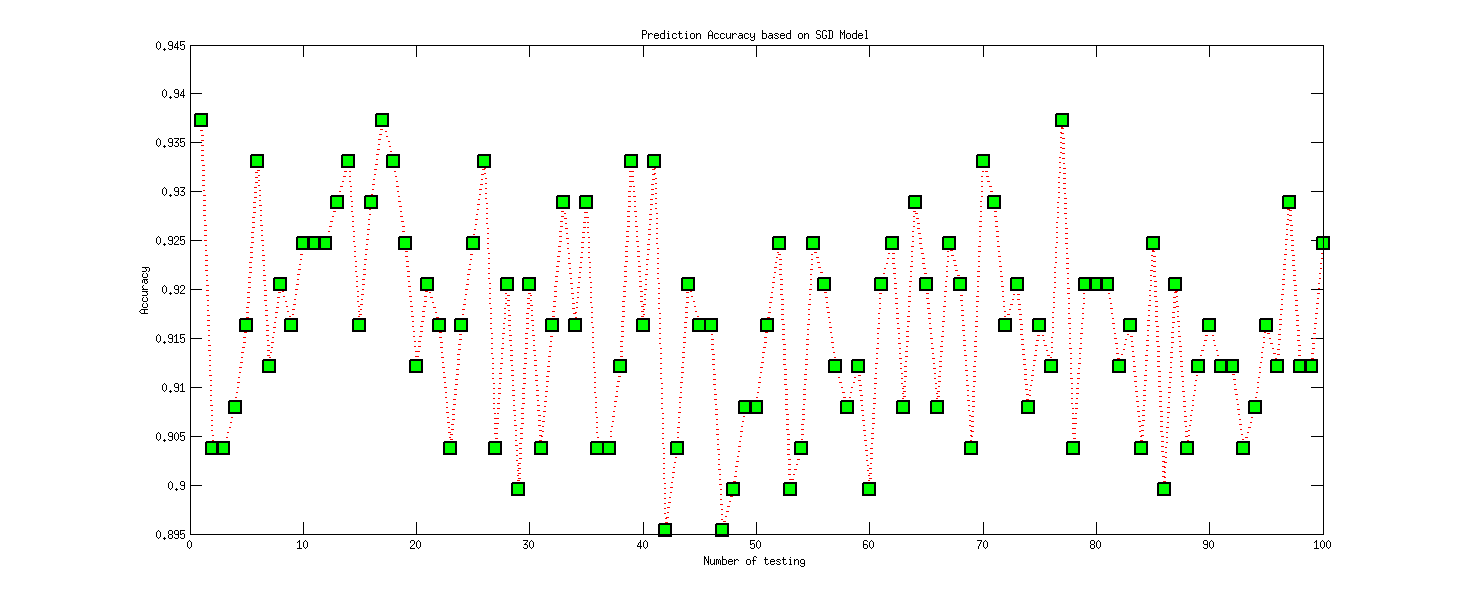
\includegraphics[width=\textwidth]{Accuracy_SDG.png}
\caption{Test set accuracy on stochastic gradient descent model.}
\label{fig:accuracy_sdg}
\end{figure}

%-----------------------------------------------------------------------------
% FINDINGS AND LESSONS LEARNED
%-----------------------------------------------------------------------------
\section{Findings and Lessons Learned}
\label{sec:conclusion}

% TODO: data is too small. Different runs can give very
% different results. For training, 447 samples and we have 800 feature --> overfitting, classification learning will fail to produce a robust model.

The Gender Recognition [DCT] dataset provided by MLcomp is too small to make a good prediction.
 With only 559 examples to be divided for both training and validation set, overfitting problem becomes unavoidable.
 Figure~\ref{fig:acc_numtrain} shows accuracy of training and validation set after training with $\lambda$ of 0.01 and $\mu$ of 0.01.
 The accuracy of training set is always 1, which clearly indicates overfitting.
 The accuracy of the validation set has to be interpreted carefully, because bigger training set means smaller validation set.
 With 500 training examples, the validation set only has 59 examples, which is too small to have a reliable accuracy calculation.
 This can explain the drop in validation accuracy at that point.

\begin{figure}[!ht]
\begin{center}
    \includegraphics[height=0.25\textheight]{acc_numtrain.jpg}
    \caption{Accuracy of both training and validation set given different size of training examples, with $\lambda$ of 0.01 and $\mu$ of 0.01.}
    \label{fig:acc_numtrain}
\end{center}
\end{figure}

The penalty added by the $L_2$ regularization can help this overfitting problem. However, there is a trade-off betw
Recompile Logs 1 Download
een maximizing likelihood and reducing overfitting.
 From figure~\ref{fig:acc_mu}, we notice that a big value of $\mu$ reduces down the accuracy of the training set.
 Whereas small values of $\mu$ seem to give similar accuracy.
 This is why we pick $\mu$ to be 0.01, as it gives a good regularization such that $\beta$ values are reasonable, without sacrificing the accuracy too much.

\begin{figure}[ht!]
\begin{center}
    \includegraphics[width=1.0\textwidth]{acc_vs_mu.jpg}
    \caption{Variance of validation set accuracy with different regularization strength $\mu$, and $\lambda$ set at 0.01.}
    \label{fig:acc_mu}
\end{center}
\end{figure}

By definition, the learning rate $\lambda$ in stochastic gradient descent affects how fast the function converges.
 However, since this optimization method only provides a local extrema point, $\lambda$ can also impact the accuracy of the trained model.
 Figure~\ref{fig:rlcl_epoch} shows how 2 different $\lambda$ values can result in 2 very different RLCL values.
 This can happen when the jump step is big enough that it overshoots from one local extrema to the next.
 However, this jump is not guaranteed to give better result. That is why choosing the $\lambda$ value is not a trivial matter, as well as choosing a good initial guess of the parameter.


\begin{figure}[!h]
\begin{center}
    \includegraphics[height=0.3\textheight]{rlcl_vs_epoch.jpg}
    \caption{Different convergence RLCL values are observed from different values of $\lambda$.}
    \label{fig:rlcl_epoch}
\end{center}
\end{figure}

% time complexity: SGD takes 87s, L-BFGS takes 38s, for 100 runs.
The average time required to train the SGD model until convergence is 0.87 seconds, whereas L-BFGS averages around 0.38 seconds.
 One reason for the slow convergence of SGD can be attributed to the small value of $\lambda$.
 However, looking at Figure~\ref{fig:rlcl_epoch}, with $\lambda$ value of 0.01 we can see that by 10 epochs, the RLCL has pretty much converged to a value, but the computation keeps going for 40 more epochs. This shows that our chosen threshold of $10^{-3}$, used to check convergence, is too small.

Overall, our SGD model, with a test error of 0.0836, seems to be performing well, even with the limitation in training set size. In fact, we achieve similar accuracy as the {\tt svmlight-linear} model with test error of 0.084 reported in MLcomp website. However, the {\tt svmlight-linear} model performs much faster at 0.16 seconds, around 5x the speed of SGD.



%-----------------------------------------------------------------------------
% BIBLIOGRAPHY
%-----------------------------------------------------------------------------
\begin{thebibliography}{1}

\bibitem{DCTdata} Gender Recognition [DCT] dataset. Available at {\tt http://mlcomp.org/datasets/1571}.

\bibitem{wiki_classifier} Wikipedia article {\em Binary classification}. Available at {\tt http://en.wikipedia.org/wiki/Binary\_ classification}.

\bibitem{wiki_lbfgs} Wikipedia article {\em Limited-memory BFGS}. Available at {\tt http://en.wikipedia.org/wiki/ Limited-memory\_BFGS}.

\bibitem{minFunc} Schmidt, M. (2012). {\em minFunc}. Available at {\tt http://www.di.ens.fr/\~mschmidt/Software/ minFunc.html}

\bibitem{elkan} Elkan, C. (2014). {\em Maximum Likelihood, Logistic Regression, and Stochastic Gradient Training}. Available at {\tt http://cseweb.ucsd.edu/$\sim$elkan/250B/logreg.pdf}.

\bibitem{checkgrad} Rasmussen, C. (2001). {\em checkgrad.m}. Available at {\tt http://learning.eng.cam.ac.uk/carl/ code/minimize/checkgrad.m}.

\end{thebibliography}

\end{document}u
